\section{Grundlagen}
Im folgenden Kapitel werden die theoretischen Grundlagen behandelt, die für das Verständnis dieser Arbeit notwendig sind. Dabei geht es in erster Linie um allgemeine Begrifflichkeiten aus dem wirtschaftlichen Kontext des zu entwickelnden Programms.

\subsection{ERP-Systeme}
ERP ist ein Akronym für den englischen Begriff \glqq{}Enterprise Ressource Planning\grqq{}, also das Planen von Unternehmensressourcen, unter anderem in den Bereichen Beschaffung, Produktion, Vertrieb, Personalwirtschaft und Finanzwesen. \footcite[Vgl.][523]{wibuch} Ein ERP-System beschreibt somit eine Software, die Prozesse aus diesen Bereichen in einem Anwendungspaket integriert und die dabei anfallenden Daten in einer zentralen Datenbank abspeichert. Dadurch werden Redundanzen in der Datenhaltung vermieden und die Umsetzung von bereichsübergreifenden Unternehmensprozessen ermöglicht \footcite[Vgl.][523]{wibuch}. ERP-Systeme nutzen in der Regel eine Client-Server-Architektur und sind komponentenorientiert, das heißt, Unternehmen können, je nach Anforderungen ihrer Wertschöpfungsprozesse, die benötigten Komponenten frei wählen. Dadurch ist eine schrittweise Einführung der ERP-Software, über einen längeren Zeitraum, möglich. \footcite[Vgl.][524 f.]{wibuch}

\subsection{SAP}
\subsubsection{Die SAP SE}
Die SAP SE wurde im Jahr 1972 von fünf ehemaligen IBM-Mitarbeitern unter dem Namen \glqq{}\underline{S}ystem\underline{a}nalyse und \underline{P}rogrammentwicklung GbR\grqq{}\footcite[Vgl.][]{think-ing}  mit dem Ziel gegründet, eine Standardanwendungssoftware für die Echtzeitverarbeitung zu entwickeln.  Im Jahr 1973 wurde durch die SAP mit dem \glqq{}System RF\grqq{} das erste Produkt für die Finanzbuchhaltung vorgestellt, was den Grundstein für die erste SAP-Generation \glqq{}SAP R/1\grqq{} legen sollte. Durch die ständigen Weiterentwicklungen wurde das System stets erweitert und fand bei immer mehr Kunden Anklang. 1976 wurde die Gesellschaft bürgerlichen Rechts aufgelöst und in eine GmbH überführt. Im selben Jahr wurde bereits mit nur 25 Mitarbeitern ein Umsatz von 3,81 Mio. DM erzielt. \footcite[Vgl.][]{sap-fruehejahre}\\Im Jahr 1979 folgt schließlich die zweite Produktgeneration \glqq{}SAP R/2\grqq{}, die eine höhere Stabilität mit sich brachte und in weitere Geschäftsbereiche vordrang. In der Generation R/2 waren bereits die Module RF für Finanzbuchhaltung, RK für die Kostenrechnung, RM für Materialwirtschaft, Produktionsplanung und Instandhaltung, RP für die Personalwirtschaft und RV für den Vertrieb verfügbar.\footcite[Vgl.][]{bewerbungsratgeber}\\Im Jahr 1988 wurde die SAP GmbH schließlich in eine Aktiengesellschaft überführt und startete an der Börse Frankfurt sowie in Stuttgart. Im selben Jahr erwirtschaftetet SAP bereits einen Umsatz von 245 Mio. DM und hatte bereits 940 Mitarbeiter. Bereits zu diesem Zeitpunkt war die dritte Generation \glqq{}SAP R/3\grqq{} in Entwicklung, die schließlich im Jahr 1992 erschien und, in Gegensatz zu ihren Vorgängern, die als Mainframe-Anwendungen liefen, auf einer Client-Server-Architektur aufgebaut war. Das führte dazu, dass SAP immer erfolgreicher wurde und auch international immer weiter expandierte, sodass im Jahr 1997 schließlich 1,6 Mrd. DM  Umsatz erwirtschaftet wurden. 1995 begann SAP damit, seine Vertriebsaktivitäten im deutschen Mittelstand auszubauen, da zuvor die Hauptkundenzielgruppe nur größere Unternehmen waren. In den darauffolgenden Jahren startete die SAP zusammen mit Microsoft seine Internetstrategie und setzte mit \glqq{}mySAP.com\grqq{} vermehrt den Fokus auf E-Commerce und E-Business-Lösungen und seit dem Jahr 2007 auch auf Business Intelligence.\footcite[Vgl.][]{sap-fruehejahre} Ab dem Jahr 2009 richtete sich die SAP verstärkt auf die Bereiche der Datenbanktechnologie und Cloud Computing aus, woraus schließlich im Jahr 2011 die Datenbanktechnologie \glqq{}SAP HANA\grqq{} entstand, die vor allem Geschwindigkeitsoptimierungen in der Datenverarbeitung mit sich brachte. 2015 wurde schließlich die vierte, heute noch aktuelle, SAP-Generation \glqq{}SAP S/4HANA\grqq{} vorgestellt, die vollständig auf SAP S/4HANA basiert und eine moderne Benutzeroberfläche mit sich bringt, mit der Anwendungen auch auf mobilen Endgeräten dargestellt werden können. Auch bietet die SAP mit S/4HANA erstmalig Cloud-Lösungen für ihre Kunden, was besonders auf kleine und mittelständische Unternehmen abzielt.\footcite[Vgl.][]{sap-historie}\\ Im Jahr 2020 belief sich der Gesamtumsatz der SAP SE auf 27,338 Mrd. EUR (IFRS), worauf alleine ca. 15 Mrd. EUR auf den Vertrieb von \glqq{}On-premise\grqq{} Softwarelizenzen und -Support zurückzuführen sind und ca. weitere 8 Mrd. EUR auf die Umsätze mit Softwarelizenzen und -Support aus den Cloud-Plattformen zurückgehen. Nach Abzug der operativen Aufwendungen und der Steuern blieben davon 5,238 Mrd. EUR Gewinn (IFRS).\footcite[Vgl.][S. 142]{sap2020-report} 

\begin{figure}[h!]
    \centering
    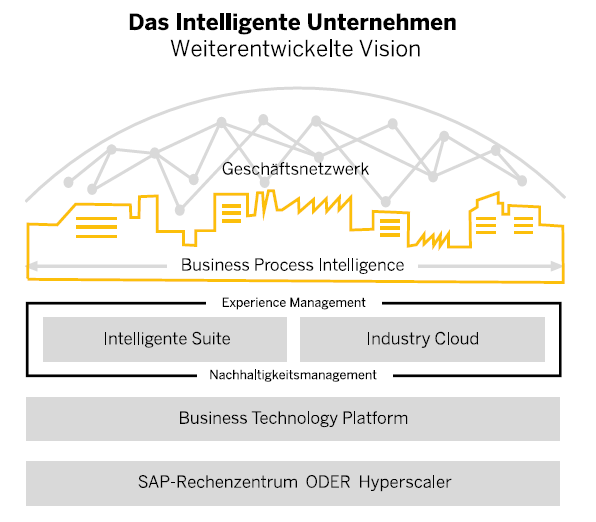
\includegraphics[scale=1]{Bilder/SAPIntelligentesUnternehmen.png}
    \caption[Das Intelligente Unternehmen]{Das Intelligente Unternehmen (Quelle: \cite[][S. 53]{sap2020-report})}
\end{figure}

Die SAP verfolgt derzeit die Vision ihre Kunden zu einem intelligenten Unternehmen zu entwickeln, in denen die Prinzipien der Innovation, Integration, Agilität und Geschwindigkeit an vorderster Stelle stehen. Außerdem alle Elemente eines Unternehmens verbunden werden und ineinandergreifen. Die Komponenten eines solchen intelligenten Unternehmens sind nach Vorstellungen der SAP ein Geschäftsnetzwerk, das die unternehmensübergreifenden Prozesse miteinander verknüpft, eine Business Process Intelligence, die die Geschäftsprozesse analysiert und optimiert, das Experience Management, das die Daten der Anwender, Kunden und Mitarbeiter analysiert, eine Business Technology Platform, die das Fundament für die Integration und Erweiterung von Anwendungen liefert und dem Kunden Möglichkeiten für künstliche Intelligenz, maschinelles Lernen und Prozessautomatisierung bietet, und einem SAP-Rechenzentrum oder einem Hyperscaler, also einem Infrastructure-as-a-Service Anbieter wie Amazons AWS oder Microsoft Azure.\footcite[Vgl.][S. 53 f.]{sap2020-report}. Dadurch soll das Ziel erreicht werden, langfristig die Abläufe der weltweiten Wirtschaft zu verbessern.


\subsubsection{SAP-ERP}
\label{kap:R3}
SAP ERP, oder auch SAP ECC (SAP ERP Central Component), ist die Weiterentwicklung der dritten Generation des SAP ERP-Systems, \glqq{}SAP R/3\grqq{}, das im Jahr 1992 die zweite Produktgeneration \glqq{}SAP R/2\grqq{} ablöste und im Jahr 2003 in \glqq{}SAP ERP\grqq{} umbenannt wurde.\footcite[Vgl.][]{sap-unterschiede} Der Name setzt sich dabei aus dem \glqq{}R\grqq{} für den Begriff \glqq{}Realtime\grqq{}, also Echtzeit, für die Echtzeitdatenverarbeitung und der \glqq{}3\grqq{} zum einen für die dritte Generation, aber auch für die dreischichtige Architektur, die dem System zugrunde liegt, bestehend aus Datenbank, Anwendungsserver und Client. Die dritte SAP-Generation verfügt dabei über eine zentrale Datenbank, in der alle Daten aus den einzelnen Modulen und den verteilten Anwendungen gesichert werden. SAP ERP bzw. SAP ECC stellt die zentrale Komponente der \glqq{}SAP Business Suite\grqq{} dar, in der noch andere Produkte von SAP erhältlich sind, die auf andere Anwendungsbereiche als ERP abzielen, aber mit denselben Daten arbeiten, zum Beispiel dem CRM (Customer Relationship Management) oder dem SCM (Supply Chain Management).\footcite[Vgl.][]{mindsquare-sap} Durch die unterschiedlich ausgerichteten Systeme können sich die Kunden ihre Systemlandschaft frei zusammenstellen und diese spezifisch an ihr Geschäftsmodell anpassen. Dadurch wird eine noch tiefer gehende Integration von Geschäftsprozessen ermöglicht, da all diese Systeme mit derselben, zentrale Datenbanken arbeiten. Die aktuellste SAP-ERP Version ist das Enhancementpackage 8 für SAP ERP 6.0 und ist im Jahr 2016 erschienen, da \glqq{}SAP R/3\grqq{} seit 2015 durch die neuste Generation \glqq{}SAP S/4HANA\grqq{} abgelöst wurde.\footcite[Vgl.][]{sap-version}\\ SAP bietet für das Grundsystem unterschiedliche Modulen an, die das System erweitern und ebenfalls durch die Kunden frei, nach ihren jeweiligen Anforderungen, zusammengestellt werden können.

\begin{figure}[h!]
    \centering
    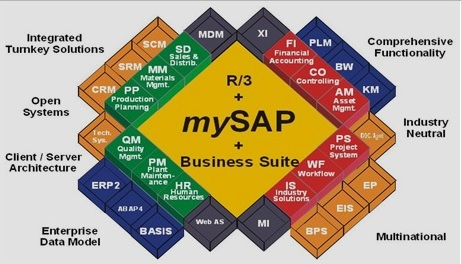
\includegraphics[scale=1]{Bilder/sap-module.jpg}
    \caption[Die Module von SAP-ERP]{Die für SAP-ERP erhätlichen Module (Quelle: \cite[][]{sap-module})}
    \label{fig:sapmodule}
\end{figure}

In der Abbildung \ref{fig:sapmodule} sind die für SAP-ERP erhältlichen Module und die dazugehörigen Anwendungen bzw. Systeme abgebildet. Die wichtigsten Module und gleichzeitig den Kern des Systems stellen dabei die Module FI, CO, MM, SD, PP und HCM dar, die zum Teil auch standardmäßig in jeder SAP-Installation vorinstalliert sind.\footcite[Vgl.][S. 8]{sap-für-wp} Auf der rechten Seite der Abbildung \ref{fig:sapmodule} sind im inneren Kreis der äußeren Umrandung der Raute, in Rot, die Module des Rechnungswesens dargestellt, FI für das externe Rechnungswesen und CO für das Controlling, bzw. das interne Rechnungswesen sind dabei am weitesten verbreitet. Auf der linken Seite sind in Grün die Logistikmodule zu sehen, bei denen PP für die Produktion, MM für die Materialwirtschaft, SD für den Vertrieb und PM für die Instandhaltung im Vordergrund stehen. Als dritte Kategorie kommt in den aktuellen Versionen von SAP ERP noch das Modul Human Capital Management (HCM) für die Personalwirtschaft dazu, das das HR-Modul abgelöst hat.\footcite[Vgl.][]{sap-module2} Im äußeren Kreis der äußeren Umrandung der Raute sind in Blau die Module der SAP Business Suite dargestellt und in Orange die zusätzlich erhältlichen SAP-Produkte, für CRM, SCM, etc.\footcite[Vgl.][]{sap-module}
\\Mit der Vorstellung der neusten SAP Generation \glqq{}SAP S/4HANA\grqq{} hat SAP angekündigt, die Unterstützung, in Form von Updates und Fehlerbehebungen, von SAP-ERP nach 10 Jahren, also im Jahr 2025, einzustellen und nur noch die neuste Generation, S/4HANA, zu unterstützen. Aufgrund der weiten Verbreitung von SAP-ERP und einer durch die Abkündigung entfachter Debatte hat die SAP angekündigt, die Kernanwendungen von SAP-ERP noch bis 2027 zu unterstützen und bis 2030, gegen Aufpreis, eine erweiterte Unterstützung anzubieten. Mit dieser Maßnahme möchte die SAP erreichen, dass alle Unternehmen in den nächsten Jahren auf die neuste Generation umsteigen.\footcite[Vgl.][]{sap-support}

\subsubsection{SAP HANA}
\label{kap:HANA}
SAP HANA ist eine sogenannte \glqq{}In-Memory\grqq{}-Datenbanktechnologie, die eigens durch die SAP für ihre Produkte entwickelt wurde, mit der große Datenmengen schnell ausgewertet werden können. Die Abkürzung HANA steht dabei für \glqq{}Hyper Perfomance Analytic Appliance\grqq{}, zu Deutsch etwa \glqq{}Höchstleistungsauswertungsinstrument\grqq{}. Die Technologie wurde bereits im Jahr 2008 von SAP in Zusammenarbeit mit der Universität Stanford und dem Hasso-Plattner-Institut\footnote{Hasso Plattner ist einer der Mitbegründer der SAP} entwickelt. Die Besonderheit von HANA ist, dass es sich dabei um sogenannte \glqq{}In-Memory-Datenbanken\grqq{} und die Inhalte der Datenbank durchgehend im Hauptspeicher (RAM) geladen sind und nicht, wie bei herkömmlichen relationalen Datenbanken, nur der aktuell für die Verarbeitung benötigte Teil vom Dauerspeicher in den Hauptspeicher geladen wird.\footcite[Vgl.][]{was-hana} Dadurch sollen die Zugriffsgeschwindigkeiten bis \glqq{}[...] zu 100.000-mal schneller als bei einer Festplatte[..]\grqq{}\footcite[Vgl.][]{rz10-hana} sein. Das vollständige Laden der Datenbank bewirkt zwar, dass dadurch der Hauptspeicher stark belastet wird und durch die Datenmengen entsprechend viel Kapazität benötigt, jedoch bewirkt das Moore'sche Gesetz, dass durch das Voranschreiten der Technologien alle 18-24 Monate die mögliche Computerleistung verdoppelt wird und gleichzeitig die Preise je Speichereinheit sinken.\footcite[Vgl.][]{mooresches}\\ Da, im Gegensatz zu dem Stückweisen Laden aus dem Datenspeicher, der Zugriff aus dem Hauptspeicher deutlich schneller vonstattengeht, ermöglicht HANA somit eine verbesserte Verarbeitung von großen Datenmengen mit hoher Geschwindigkeit. So ist es Unternehmen möglich, die gesamte Datenbank in Echtzeit zu analysieren und darauf basierende Entscheidungen zu treffen, wodurch Geschäftsprozess beschleunigt und effizienter gemacht werden können. Eine weitere Besonderheit von HANA ist die Spaltenorientierung, da traditionelle, relationale, Datenbanken in der Regel zeilenorientiert arbeiten und die einzelnen Datensätze je Zeile gespeichert werden. Dadurch ist es möglich, zum Beispiel bei Auswertungen, schnell auf alle Dateneinträge eines Datenbankattributs zuzugreifen, da diese zusammen in einer Zeile gespeichert werden. Auch sind in HANA analytische und transaktionale Daten gemeinsam verfügbar und die analytischen Daten werden nicht, wie bei herkömmlichen Datenbanken, vorher repliziert. Dadurch arbeiten Analysen in HANA stets mit den aktuellen, transaktionalen, Datensätzen. Um die Schreibvorgänge zu beschleunigen, gibt es in HANA einen Puffer, der die zeilenbasiert gelieferte Daten in die benötigte Spaltenstruktur umwandelt.\footcite[Vgl.][]{was-hana}\\Ein Problem, das bei In-Memory-Datenbanken besteht, ist die Erfüllung der sogenannten ACID-Kriterien, die von Datenbanken, bzw. Datenbank-Managementsystemen erfüllt werden müssen. Das Akronym \glqq{}ACID\grqq{} steht dabei für die Eigenschaften \underline{A}tomicity (Atomarität), \underline{C}onsistency (Konsistenz), \underline{I}solation (Abgrenzung) und \underline{D}ura-bility (Dauerhaftigkeit). Von Natur aus kann die Anforderung der Dauerhaftigkeit bei der Datenhaltung im Hauptspeicher nicht gegeben werden, da dieser flüchtig ist und im Falle einer Stromunterbrechung durch einen Stromausfall, oder Systemabsturz seine Daten verliert. Um dieses Problem zu lösen, gibt es in HANA einen \glqq{}Persistenz Layer\grqq{}, der dafür sorgt, dass die Datenbank in regelmäßigen Abständen (standardmäßig 300 Sekunden) in Form von \glqq{}Savepoints\grqq{} (Sicherheitspunkten) auf einem Dauerspeicher gesichert wird. Um auch nicht beendete Transaktionen auf der Datenbank wiederherzustellen, gibt es die Möglichkeiten den letzten Zustand anhand von Logs zu rekonstruieren. Auf demselben Weg ist es auch möglich, den vorherigen Zustand nach Abbruch einer Datenbanktransaktion wiederherzustellen, wodurch zugleich auch die Eigenschaft der Konsistenz gewährleistet wird.\footcite[Vgl.][]{rz10-acid}

\subsubsection{SAP S/4HANA}
\label{kap:S4HANA} 
SAP S/4HANA ist die neuste Generation des ERP-Produkts von SAP. Mit S/4HANA wurde im Jahr 2015 die vorherige Generation SAP-ERP (R/3) abgelöst und vollstän-dig auf Basis der neuen HANA-Datenbanktechnologie (siehe Kapitel \ref{kap:HANA}) entwickelt und angepasst. Dazu kommt, dass mit S/4HANA eine neue Benutzeroberfläche für Webanwendungen eingeführt wurde, den sogenannten FIORI-Anwendungen.\footcite[Vgl.][]{was-hana} Der Name \glqq{}S/4HANA\grqq{} setzt sich dabei aus dem \glqq{}S\grqq{} für \glqq{}Suite\grqq{}, also der Anwendungssuite von SAP, der \glqq{}4\grqq{} für die vierte Produktgeneration des SAP-ERP-Systems und \glqq{}HANA\grqq{} für die bereits erwähnte Datenbanktechnologie zusammen.\footcite[Vgl.][]{rz10-s4hana}\\SAP verspricht mit S/4HANA viele Neuerungen und Vereinfachungen im System, die in sogenannten \glqq{}Simplification-Lists\grqq{} (Vereinfachungslisten) beschrieben werden. Diese Vereinfachung und Verschlankung des Systems geschieht beispielsweise durch das Zusammenlegen von bestehenden Funktionen, wie dem Verschmelzen der Kreditoren und Debitoren zu Geschäftspartnern, und durch die Reduzierung des Datenmodells, indem nicht mehr benötigte Komponenten, wie z.B. durch HANA überflüssig gewordene Aggregationstabellen, entfernt werden. Dies hat jedoch den Nachteil, dass der Umstieg auf S/4HANA viele Hürden mit sich bringt, da vieles bei einer Datenmigration nicht eins zu eins übernommen werden kann.\footcite[Vgl.][]{ibsolution}\\Eine weitere Neuerung von S/4HANA ist die Vermarktung entweder als Cloud-Lösung oder, wie bisher, als On-Premise-Lösung, also als klassische Installation auf einem vom Unternehmen gestellten Server. Die Cloud-Lösung bietet SAP S/4HANA sowohl als \glqq{}Public Cloud\grqq{}-Lösung auch als \glqq{}Private Cloud\grqq{}-Lösung an.
\begin{figure}[h]
    \centering
    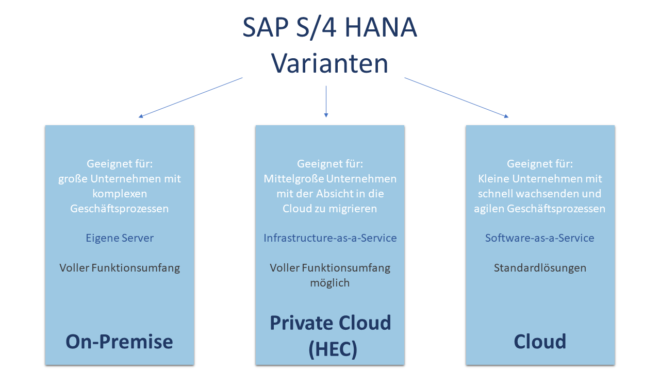
\includegraphics[scale=1.3]{./Bilder/HANA-Varianten.png}
    \caption[S/4HANA Lösungen]{Angebotene Lösungsvarianten von S/4HANA (Quelle: \cite[][]{rz10-s4hana})}
\end{figure}
\\Mit der Public-Cloud bietet die SAP ihre ERP-Lösung erstmalig als Software-as-Service (SaaS)-Produkt an, was zur Folge hat, dass der Kunde sich weder um die Bereitstellung der benötigten Hardware, die Installation noch der Aktualisierung der Software kümmern muss, da dieses zentral durch die SAP auf den SAP-eigenen Servern geschieht. Dies hat zum einen für die SAP den Vorteil, dass sie schnell Fehler beheben und Aktualisierungen ausrollen können, die direkt für die Kunden verfügbar sind, ohne, dass diese erst einen Patch oder ein Funktion-Update einspielen müssen. Auch lässt sich die Lizenzierung des Produkts vereinfachen, indem der Kunde nun per Benutzerzugang zahlt und nicht mehr für eine Softwarelizenz. Für die Kunden bringt eine solche Cloud-Lösung ebenfalls Vorteile mit sich, da, wie bereits oben erwähnt, keine eigene Hardware mehr vorgehalten und gewartet werden muss. Dazu kommt, dass die erstmalige Inbetriebnahme des Systems vereinfacht wird, da auch kein Aufsetzen des Servers und keine Installation der Software erfolgt, sondern die Zugänge in der Regel online gebucht und anschließend direkt genutzt werden können. Außerdem ist mit einer solchen Lösung die IT-Sicherheit des ERP-Systems verbessert, da der Kunde sich nun nicht mehr selbst um Backups, Systemupdates oder Systemredundanzen kümmern braucht, sondern die Verantwortung auf den Serviceprovider, also die SAP, abgegeben wird.\footcite[Vgl.][]{saas} Die SAP-Public Cloud hat jedoch den Nachteil, dass sich viele unternehmensspezifische Anpassungen und Eigenentwicklungen, die als \glqq{}Customizing\grqq{} in der Branche weitverbreitet sind, nicht durchführen lassen, da die Public Cloud als reine Standardlösung angeboten wird. Die SAP richtet sich mit dem Produkt dadurch vor allem an kleine und mittelständische Unternehmen, die zum einen durch den geringen Aufwand profitieren, auf der anderen Seite aber auch keine Einbußen durch fehlende Eigenentwicklungen und Anpassungsmöglichkeiten haben.\footcite[Vgl.][]{rz10-s4hana}\\Die Private-Cloud-Lösung von S/4HANA (als \glqq{}HANA Enterprise Cloud (HEC)\grqq{} von SAP vermarktet), bringt die Vorteile der Public Cloud mit sich, ermöglicht aber auch Customizing und Eigenentwicklungen. Dies geschieht, indem der Kunde, mit dem Produkt der Private-Cloud, einen eigenen Server bei der SAP anmietet, sich aber dennoch nicht um die Wartung, Aktualisierung, etc. kümmern muss, da dies wie bei der Public-Cloud durch den Serviceprovider geschieht. Die SAP richtet sich mit dem Angebot vor allem an Unternehmen, die bereits SAP eingeführt haben und bereit sind in die Cloud zu wechseln, aber nicht auf ihre eigenen Systemanpassungen, Abweichungen vom Standard, verzichten möchten, bzw. können.\footcite[Vgl.][]{rz10-hana}\glqq{}Die HEC ist eine End-to-End-Lösung, die eine umfassende Cloud-Infrastruktur und Managed Services für In-Memory-Anwendungen, Datenbanken und Plattformen bietet.\grqq{}\footcite[Vgl.][]{rz10-hana}\\Die Dritte, von SAP angebotene S/4HANA-Variante, ist die On-Premise Lösung (Vorort-Lösung), die der Lösungsvariante der vorherigen SAP Generation entspricht. Hierbei wird der Server durch den Kunden selbst gestellt und dieser ist somit selbst für die Installation, Wartung und Sicherheit verantwortlich.\footcite[Vgl.][]{rz10-s4hana} Das ermöglichtet dem Kunden eine größtmögliche Flexibilität, birgt aber Risiken durch etwaige Sicherheitslücken, Systemausfällen oder Datenverlust. Auch ist im Vergleich zu den vorherigen Generationen die Anforderungen an die benötigte Server-Hardware gestiegen, da durch die neue HANA-Datenbank mehr Arbeitsspeicher benötigt wird (siehe Kapitel \ref{kap:HANA}). Die SAP richtet sich mit der On-Premise-Lösung vorwiegend an größere Unternehmen und Konzerne, die bereits SAP in der Benutzung haben und keine Änderungen an ihrer Infrastruktur und den Prozessen zur Systempflege und Wartung vornehmen möchten.  

\subsection{Transformation}
\subsubsection{Definition}
Unter einer Transformation versteht man im Allgemeinen einen grundlegenden Wandel, der durch bestimmte Faktoren, wie z.B. einer sprunghaft wirtschaftlichen, oder technologischen Entwicklung hervorgerufen wird. Die Transformation hält dabei in der Regel über einen längeren Zeitraum an und ist erst beendet, sobald sich die neu geschaffenen Strukturen etabliert und gefestigt haben.\footcite[Vgl.][]{difu}\\ Im betriebswirtschaftlichen Kontext versteht man unter einer Transformation (oder auch Business Transformation) die gezielte Umgestaltung eines Unternehmens und seiner Geschäftsprozesse, um auf veränderte Bedingungen am Markt einzugehen und sich ihnen anzupassen. Dabei ist das Ziel durch effizientere und vereinfachte Geschäftsprozesse einen Mehrwert in Form von niedrigeren Kosten bei gleichbleibender, oder bestenfalls verbesserter Qualität zu erreichen und dabei zusätzlich die Kundenzufriedenheit zu steigern.\footcite[Vgl.][]{leanix}

\subsubsection{Die vier R der Transformation}
In den 1990er-Jahren wurde durch Gouillart und Kelly das Modell der \glqq{}Vier R der Transformation\grqq{} \footcite[Vgl.][]{4r-modell} entwickelt, was eine mögliche Form der Business-Transformation darstellen soll. Aus diesem Modell hat die Beratungsgesellschaft Gemini Consulting (später in der Capgemini SE aufgegangen)\footcite[Vgl.][]{gemini-died} ein Produkt entwickelt, indem die vier R für vier verschiedene Transformationsdimensionen stehen:\\
\begin{figure}[h]
    \centering
    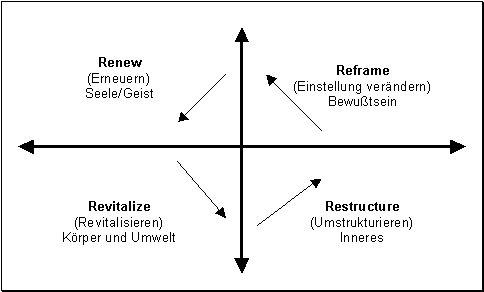
\includegraphics[scale=0.5]{Bilder/businesstransformationManagementportal.png}
    \caption[Die vier R der Transformation]{Die vier R der Transformation (Quelle: \cite[][]{4r-modell})}
\end{figure}
\begin{itemize}
    \item[] \emph{Reframing (dt. Einstellungsveränderung):} soll in einem Unternehmen dazu beitragen, die Sichtweise auf sich selbst zu überdenken, um sich dadurch von alten Denkmustern zu befreien. Um diese Einstellungsveränderung anzustoßen, ist es wichtig, dass die Mitarbeiter motiviert werden und davon überzeugt sind durch die eingesetzte Energie einen Mehrwert zu generieren. Im nächsten Schritt muss anschließend eine Vision definiert werden, die sich erheblich von der präsenten Realität absetzt um im Anschluss daraus Ziele und Messgrößen zu entwickeln. 
    \item[] Mit der \emph{Restructuring (dt. Restrukturierung)} oder auch Umstrukturierung soll der Aufbau eines Unternehmens überdacht werden, mit dem Ziel durch die Maßnahme eine Verschlankung zu erreichen und dadurch effizienter zu werden. Dies kann durch das Zusammenlegen von Abteilungen, aber auch durch Fluktuation erreicht werden. Im Anschluss ist es notwendig, ebenfalls die Geschäftsprozesse an die neue Struktur anzupassen.   
    \item[] \emph{Revitalising (dt. Wiederbelebung):} Mit der Revitalisierung soll Wachstum erzielt werden, indem sich genauer auf die Kunden ausgerichtet wird und die Erfüllung der Kundenbedürfnisse weiter in Mittelpunkt legt. Eine weitere Option für das Erreichen einer Revitalisierung ist die Erprobung neuer Geschäftsfelder um sich dadurch neue Kunden zu erschließen und Wachstum zu generieren.
    \item[] \emph{Renewing (dt. Erneuerung):} zielt schließlich auf die Mitarbeiter des Unternehmen ab, die sich zum einen mit der neuen Situation vertraut machen sollen, zum anderen, aber auch neue, nun benötigte, Fähigkeiten zu erlernen, um das Unternehmen in seiner neuen Situation voranzubringen. Dazu ist es wichtig, Reize für die Mitarbeiter zu schaffen, diesen Weg zu gehen.
\end{itemize}

\subsection{SAP S/4HANA Transformation}
\label{kap:s4hanatrans}
Die S/4HANA Transformation stellt eine besondere Art der Transformation dar, da sie einen Umstieg auf die neuste SAP Generation in Kombination mit einer digitalen Transformation ermöglicht. Diese Möglichkeit besteht, da die vielen Neuentwicklungen und Vereinfachungen in S/4HANA viel Aufwand für die Aktualisierung des Systems bedeuten, aber gleichzeitig ein großes Potential an Möglichkeiten zur Optimierung der abgebildeten Prozesse ermöglichen. Dadurch wird ein umfassender, innerbetrieblicher Wandel, hin, zu einem digitalisierten Unternehmen mit intelligenten Geschäftsprozessen ermöglicht, unterstützt durch die Echtzeit-Auswertungen und den Möglichkeiten der Business Intelligence, die S/4HANA bietet.
\\Aufgrund der langen Laufzeit von SAP-ERP, bzw. R/3, das seit Beginn der 1990er-Jahre verfügbar war, gibt es viele Systeme, die bereits sehr lange im Einsatz und somit sich historisch gewachsen sind. Während dieser Entwicklung wurden die Systeme immer weiter an die Erfordernisse des jeweiligen Unternehmens angepasst, sodass teils ein großes Delta zum Industriestandard entstanden ist. Mit einer S/4HANA-Transformation ist es nun möglich, alle Geschäftsprozesse zu überdenken und zu optimieren, sowie weitere Geschäftsprozesse zu digitalisieren, da über die Jahre der Funktionsumfang, und somit die Möglichkeit der Abbildung von Geschäftsprozessen, von SAP-ERP stark angewachsen ist und somit, im Vergleich zum Zeitpunkt der Einführung der meisten Systeme, sich viel mehr Möglichkeiten ergeben, Prozesse zu digitalisieren.\footcite[Vgl.][]{s4-interview}
\\Dazu ist es wichtig, sich im Vorfeld mit der eigenen Unternehmensvision und -strategie auseinanderzusetzen, und auf Basis derer, Entscheidungen über die angestrebte Prozesslandschaft und das Betriebsmodell zu treffen. Dadurch ist man in der Lage, den möglichst besten Transformationspfad zu beschreiten und die Lösung für seine Probleme, zu einem bestmöglichen Kosten/Nutzen-Verhältnis, zu erzielen.\footcite[Vgl.][]{ao-blog}
Zur Durchführung einer S/4HANA-Transformation gibt zwei von SAP vorgestellte Ansätze, die zwei Extremwege vertreten. Zum einen ist das der Greenfield-Ansatz (Aufbau auf der \glqq{}Grünen Wiese\grqq{}) und zum anderen der Brownfield-Ansatz (Aufbau auf dem Altsystem). Des Weiteren gibt es noch verschiedene hybride Ansätze, die einen Mittelweg zwischen Greenfield und Brownfield darstellen.\footcite[Vgl.][]{ao-blog} Diese Ansätze werden in den folgenden Unterkapiteln genauer behandelt.
%Industrie 4.0
\subsubsection{Greenfield Ansatz}
Der Greenfield-Ansatz sieht einen kompletten Neuaufbau des SAP ERP-Systems vor und baut nicht auf dem R/3-System auf, sodass dieses bis zur Fertigstellung des neuen Systems in Betrieb bleibt. In der neuen S/4HANA-Installation wird währenddessen ein komplett neues System geschaffen, in dem alle abzubildenden Geschäftsprozesse komplett neu gedacht werden und das Geschäftsmodell des Unternehmens angepasst wird.\footcite[Vgl.][]{ao-blog} Dabei wird das Ziel verfolgt, möglichst die \glqq{}Best Practices\grqq{} des Industriestandards zu implementieren und auf Eigenentwicklungen zu verzichten, um im Nachhinein den Wartungsaufwand so gering wie möglich zu halten. Eigenentwicklungen und unternehmenseigene Workarounds sind in der SAP-Branche weit verbreitet, haben jedoch den Nachteil, dass sie hohe Wartungskosten und einen hohen Pflegebedarf mit sich bringen und auch nicht besonders effizient im Umgang mit der HANA-Datenbank sind und dadurch oftmals auch nicht von den S/4HANA-Verbesserungen profitieren können.\\Im Zuge einer Greenfield-Transformation wird auch das Umfeld des SAP-Systems neu bewertet und Umsysteme bei schlechtem Kosten/Nutzen-Verhältnis abgelöst. Dabei wird auch untersucht, ob die Systeme inzwischen redundant sind und durch den SAP-Standard abgelöst werden können. Die Greenfield-Transformation stellt einer der wenigen Chancen dar, das komplette ERP-System neu aufzubauen und die darin enthaltenen Prozesse neu zu denken, da die moderne Softwareentwicklung sich immer weiter von großen, gebündelten Patches entfernt und mehr in die Richtung von kontinuierlichen, inkrementellen Updates geht und somit stetig der Funktionsumfang wächst.\footcite[Vgl.][]{gambit-transformation} Dies ist vor allem in den S/4HANA-Cloud-Lösungen der Fall, da hier die Systeme und die Software durch die SAP betrieben und gewartet werden und somit Aktualisierungen noch einfacher durchgeführt werden können (siehe Kapitel \ref{kap:S4HANA}). Im Vergleich zum Brownfield-Ansatz ist der Aufwand einer Greenfield-Transformation sehr hoch, da die Implementierung der neuen Prozesse viel Zeit benötigt und die neuen Prozesse auch nach der Einführung getestet werden müssen, ob sie die Anforderungen des Unternehmens abdecken. Auch ist es essentiell, dass die Benutzer, durch Schulungen, in das neue System und die neuen Prozesse eingeführt werden, da es hier zu gravierenden Unterschieden in den Arbeitsabläufen kommen kann.\footcite[Vgl.][]{gambit-transformation} Dies stellt einen zusätzlichen Aufwand dar, der mit einer Brownfield-Transformation vermieden werden kann.

\subsubsection{Brownfield Ansatz}
Der Brownfield-Ansatz basiert auf der Überlegung, auf dem bestehenden SAP-ERP-System der dritten Generation aufzubauen und es nach S/4HANA zu konvertieren. Dazu werden die bestehenden und bereits abgebildeten Prozesse nach S/4HANA übertragen und nicht, wie im Greenfield-Ansatz, komplett neu aufgebaut. Dies bietet für die Unternehmen eine schnellere Implementierung, da die bestehenden Strukturen nur angepasst werden müssen und historischen Daten und Eigenentwicklungen erhalten bleiben. Auch bietet dieser Ansatz Vorteile für die Anwender des Systems, da diese sich nicht auf neue Prozesse einstellen müssen, sondern ihre verinnerlichten Arbeitsabläufe weiterhin anwenden können. Dadurch kann nach Abschluss der Transformation mit der selben Effizienz weitergearbeitet werden und es kommt zu weniger Fehlern.\footcite[Vgl.][]{gambit-transformation}
\\Die Nachteile des Brownfield-Ansatzes sind jedoch, dass die historisch gewachsene Komplexität des Systems mit all seinen Eigenentwicklungen und Workarounds erhalten bleibt und das volle Potential von SAP S/4HANA nicht genutzt werden kann. Auch bleibt dadurch eine Annäherung an die Best Practices des Industriestandards aus, da eine Bewertung der Prozesse, der Eigenentwicklungen und der Umsysteme nicht stattfindet, was eine unveränderte, oder im schlimmsten Fall, eine Steigerung der Betriebs- und Wartungskosten bedeutet, da die Möglichkeit bestehen, dass diese nicht gut mit S/4HANA harmonieren. Außerdem ist die Nutzung der Public-Cloud-Lösung mit dem Brownfield-Ansatz in der Regel nicht möglich, da diese keine Möglichkeit für Eigenentwicklungen und tiefgreifende Anpassungen bietet, sondern nur die Standardprozesse abbildet. Aus diesen Gründen richtet sich der Brownfield-Ansatz vor allem an Unternehmen, die ihr SAP-ERP noch nicht lange in Betrieb haben, nah am Industriestandard ihrer Prozesse arbeiten und dadurch kaum Eigenentwicklungen und historische \glqq{}Altlasten\grqq{} haben.\footcite[Vgl.][]{gambit-transformation}

\subsubsection{Hybride Ansätze}
Als dritte Möglichkeit bieten viele Beratungsunternehmen einen eigenen, hybriden Ansatz an (teilweise auch \glqq{}Bluefield\grqq{} genannt), der die Vorzüge einer Greenfield-Transformation mit denen einer Brownfield-Transformation vereinen soll. Diese Ansätze unterscheiden sich von Beratungsunternehmen zu Beratungsunternehmen, basieren jedoch zumeist auf der Neuaufsetzung eines S/4HANA-Systems mit einer anschließenden Migration der benötigten Daten. In diesem System werden dann die S/4HANA-bezogenen Anpassungen vorgenommen. Die bestehenden Prozesse und Entwicklungen im Altsystem werden bewertet und mit ins neue System übernommen, wenn sie essentiell sind und nicht durch den SAP-Standard abgelöst werden können. Diese hybriden Ansätze haben den Vorteil, dass historische Daten übernommen werden können und flexibel entschieden werden kann, welche bestehenden Strukturen übernommen werden. Somit kann dies ganz nach Wunsch der Kunden geschehen und es kann dennoch, wenn auch nur in Teilen, von den Vorzügen S/4HANAs profitiert werden.\footcite[Vgl.][]{hybrideransatz}\\
Im späteren Verlauf dieser Arbeit wird noch einmal genauer auf das Vorgehensmodell zu einem hybriden Ansatz der \glqq{}adesso orange AG\grqq{} eingegangen.
